\documentclass[conference]{IEEEtran}

\usepackage{booktabs} % For formal tables
\usepackage{pgfplots}
\usepackage{algorithmic}
\usepackage{algorithm}
\usepackage{amsmath}
\usepackage{amssymb}
\usepackage{amsfonts}
\usepackage{balance}
\usepackage{epsfig}
\usepackage{graphicx}
\usepackage{multirow}
\usepackage{xspace}
\usepackage{url}
\usepackage{color}
\usepackage {balance}
\usepackage{eqparbox}
\usepackage{mathrsfs}
\usepackage{caption}
\usepackage{subcaption}
\usepackage{lipsum}
\usepackage{enumitem}
\usepackage{float}
\usepackage{array, multirow}
\usepackage{balance}
\usepackage{hyperref}
\usepackage[utf8]{inputenc}
\usepackage{bbm}
\usepackage{bm}

\usepackage{tabularx}
\usepackage{makecell}
 %\usepackage{bickham}
        %\usepackage{boondox-cal}
        %\usepackage{boondox-calo}
       % \usepackage{dutchcal}

\captionsetup{skip=0pt}

% correct bad hyphenation here
\hyphenation{op-tical net-works semi-conduc-tor}

\newcolumntype{L}[1]{>{\raggedright\let\newline\\\arraybackslash\hspace{0pt}}m{#1}}
\newcolumntype{C}[1]{>{\centering\let\newline\\\arraybackslash\hspace{0pt}}m{#1}}
\newcolumntype{R}[1]{>{\raggedleft\let\newline\\\arraybackslash\hspace{0pt}}m{#1}}

\newtheorem{Problem}{Problem}
\newtheorem{Theorem}{Theorem}
\newtheorem{Definition}{Definition}
\newtheorem{Corollary}{Corollary}
\newtheorem{Lemma}{Lemma}
\newtheorem{Example}{Example}
\newcommand{\eat}[1]{}
\newtheorem{Assumption}{Assumption}
\newcommand{\from}[2]{{\bf [{\sc from #1:} #2]}}
\newcommand{\C}{\mbox {${\cal C}$}}

\newcommand{\tstart}{\mbox {${T_{start}}$}}
\newcommand{\tend}{\mbox {${T_{end}}$}}

\definecolor{L_color}{rgb}{0.8,0.2,0.2}
\definecolor{Y_color}{rgb}{1.0, 0.0, 0.5}
\newcommand{\LK}[1]{{\color{L_color}  #1}}
\newcommand{\Yu}[1]{{\color{Y_color} [Yu: #1]}}
\newcommand{\nop}[1]{}
\newcolumntype{Z}{ >{\centering\arraybackslash}X }

\newcommand{\algorithmicinput}{\textbf{Input:} }
\newcommand{\algorithmicoutput}{\textbf{Output:} }
\newcommand{\BertMWE}{\mbox{\sf Bert-MWE}\xspace}
\newcommand{\BertConcat}{\mbox{\sf Bert-Concat}\xspace}
\newtheorem{Principle}{Principle}



\newcommand{\red}[1]{\textcolor{BrickRed}{#1}}
\newcommand{\orange}[1]{\textcolor{BurntOrange}{#1}}
\newcommand{\green}[1]{\textcolor{OliveGreen}{#1}}
\newcommand{\blue}[1]{\textcolor{MidnightBlue}{#1}}
\newcommand{\gray}[1]{\textcolor{black!60}{#1}}

\DeclareRobustCommand{\mb}[1]{\ensuremath{\boldsymbol{\mathbf{#1}}}}

\DeclareMathOperator*{\argmax}{arg\,max}
\DeclareMathOperator*{\argmin}{arg\,min}

\DeclareMathOperator*{\diag}{diag}

\newcommand\dif{\mathop{}\!\mathrm{d}}

\newcommand{\bm}{\mathbf{m}}
\newcommand{\bs}{\mathbf{s}}

\newcommand{\bw}{\mathbf{w}}
\newcommand{\bx}{\mathbf{x}}
\newcommand{\by}{\mathbf{y}}
\newcommand{\bz}{\mathbf{z}}
\newcommand{\balpha}{\mb{\alpha}}
\newcommand{\bbeta}{\mb{\beta}}
\newcommand{\bmu}{\mb{\mu}}
\newcommand{\bsigma}{\mb{\sigma}}
\newcommand{\btheta}{\mb{\theta}}
\newcommand{\blambda}{\mb{\lambda}}
\newcommand{\bgamma}{\mb{\gamma}}
\newcommand{\bphi}{\mb{\phi}}
\newcommand{\btau}{\mb{\tau}}
\newcommand{\bvarphi}{\mb{\varphi}}
\newcommand{\bc}{\mathbf{c}}
\newcommand{\ELBO}{\textsc{elbo}}
\newcommand{\cN}{\mathcal{N}}
\newcommand{\cQ}{\mathcal{Q}}
\newcommand{\mathcalD}{\mathcal{D}}

\newcommand{\g}{\,\vert\,}
\newcommand{\E}{\mathbb{E}}
\newcommand{\EE}[1]{\mathbb{E}\left[#1\right]}
\newcommand{\EEE}[2]{\mathbb{E}_{#1}\left[#2\right]}
\newcommand{\kl}[1]{\textsc{kl}\left(#1\right)}
\newcommand{\vct}[1]{\textbf{#1}}
\newcommand{\realline}{\mathbb{R}}
\newcommand{\indpt}{\protect\mathpalette{\protect\independenT}{\perp}}
\def\independenT#1#2{\mathrel{\rlap{$#1#2$}\mkern2mu{#1#2}}}
\newcommand{\h}[1]{\textrm{H}\left( #1 \right)}
\newcommand{\half}{\frac{1}{2}}
\newcommand{\new}{\textrm{new}}
\newcommand{\mult}{\textrm{Mult}}
\newcommand{\Dir}{\textrm{Dir}}
\newcommand{\discrete}{\textrm{Discrete}}
\newcommand{\Bern}{\textrm{Bern}}
\newcommand{\DP}{\textrm{DP}}
\newcommand{\GP}{\textrm{GP}}
\newcommand{\Bet}{\textrm{Beta}}
\newcommand{\const}{\mathrm{const}}
\newcommand{\pois}{\textrm{Pois}}

\newcommand{\ddx}[1]{\frac{\partial}{\partial #1}}
\newcommand{\dfdx}[2]{\textstyle \frac{\partial #1}{\partial #2}}

\newcommand{\yrep}{y^{\textrm{rep}}}
\newcommand{\ynew}{y^{\textrm{new}}}
\newcommand{\yobs}{y^{\textrm{obs}}}
\newcommand{\model}{\mathcal{M}}
\newcommand{\ppc}{\textrm{ppc}}
\newcommand{\ideal}{\textrm{ideal}}
\newcommand{\loglik}{\mathcal{L}}
\newcommand{\nw}{\textrm{new}}
\newcommand{\data}{\mathcal{D}}

\newcommand{\Gam}{\textrm{Gam}}

\newenvironment{remark}[1][Remark]{\begin{trivlist}
\item[\hskip \labelsep {\bfseries #1}]}{\end{trivlist}}

\begin{document}
\title{
Bert-Mwe: a variational approach for non-compositionality inference in deep self attention network
}

\nop{
\author{Keqian Li}
\affiliation{\institution{University of California at Santa Barbara}}
\email{{klee}@cs.ucsb.edu}

\renewcommand{\shortauthors}{K. Li et al.}
\renewcommand{\shorttitle}{UNEC}
}

\author{\IEEEauthorblockN{Anonymous}
}

\maketitle




\begin{abstract}
The recent emergence of multi-level deep self attention neural network has revolutionized the way we model text data and use it for downstream analytical tasks. 
It works by first breaking text into single words or word pieces, 
and learning deep representation of the text based on the deep composition.
However, natural languages are not always compositional.
in that many important concepts usually correspond to atomic multi-word  expressions (MWE) such as 
idioms such as ”dog day”, named entities such as ”Palo Alto”, and technical terminologies such as ”support vector machine”,
whose meanings can not be decomposed into single word tokens and thus will be missed by the deep self-attention neural network.
In this work, we propose \BertMWE, a  principled probabilistic framework that combines the best of the deep self attention network architecture and natural language non-compositionality, 
by infusing the neural network with additional multi-world expression, and dynamically inferring their best combination via variational inference. Experiments demonstrated the effectiveness of our approach over the state of the art baseline models across a wide range of language modeling and understanding evaluation benchmarks. 
Experiments demonstrated the effectiveness of our approach over the state of the art baseline models across a wide range of text modeling and downstream analytical tasks.
\end{abstract}


%!TEX root =  concept_mining.tex


\nop{ refers to the idiosyncratic, non-composable, expression that span across different word, which includes
idioms such as "dog day", which me- ans "a period of inactivity", 
named entities such as "Palo Alto", 
or technical terms such as "generative adversarial network" \cite{sag2002multiword, baldwin2010multiword, constant2017multiword, hashimoto2016adaptive}. 
}

\section{Introduction}

%Multiword expressions (MWEs) are linguistic objects containing two or more words and showing some degree of non-compositionality. For instance, the meaning of to kick the bucket (i.e. ‘to die’) cannot be predicted from the meaning of its components, while the (masculine) gender of un peau rouge (’redskin’ in French) is not inherited from its nominal component (peau ’skin’ is feminine).
%MWEs encompass versatile linguistic objects: compounds (air brake), complex terms (random access memory), multiword named entities (European Bank for Reconstruction and Development), light-verb constructions (to take a nap), phrasal verbs (to make up for sth), idioms (to kick the bucket), proverbs (Fortune favours the bold.), etc Basic facts about MWEs are that: (i) they are prevalent in natural language texts – up to 40% of text items belong to MWEs (Gross and Senellart 1998, Sag et al. 2002);

The existence of atomic, non-composable Multi-word expressions (MWE) in text data has been widely recognized :  Jackendoff et.al. \cite{jackendoff1997architecture} estimates that 
the number of MWEs in a speaker's lexicon is of the same order of magnitude as the number of single words.
This is especially the case for specialized domain, such as terminology. 
Justenson et.al. \cite{justeson1995technical} claims that 
"when native English forms are used to create new terms, 
it most often takes at least two words to adequately specify a meaning", 
and even if the terminology is not in the form of MWE, they 
"are Greek or Latin forms made up of more than one root, e.g. aerodynamics". 
In \autoref{tab-examplar} we list some exemplar MWEs from the language modeling and understanding benchmarks dataset we use, 
which can be helpful in conveying meaning and determining the context 
to help support modeling and understanding text.
Driven these observations are extensive applications such as information retrieval \cite{xiong2015query, dalton2014entity, shen2018entity}, text classification \cite{furnkranz1998study}, machine translation \cite{koehn2003statistical}, parsing \cite{cafferkey2007multi, savary2015parseme} information extraction and knowledge base construction \cite{banko2007open, wu2012probase, ren2016automatic}, among many others.

%claims that our mental lexicon (vocabulary) of MWEs is as extensive as the one that is made up of single words, 

Despite the its wide existence,  multi-word expression has been largely overseen by deep learning approaches, 
whose typical processing pipeline goes like this:
given a piece of input text, 
we first tokenize it into a \textit{linear sequence representation} made up of single word tokens or word pieces,
and treat it as 1d sequential data to apply neural network models \cite{collobert2011natural, zhou2016attention, devlin2018bert}, which in the past 2 years, has converged towards the deep self attention networks \cite{vaswani2017attention}. 
All of these approaches rely on the assumption that the meaning of text can be captured by composing the meanings from its individual component words, 
and is thus contradicting with the existence of multi-word expressions, which are by definition ``non-composable".


\begin{table}
\centering
\caption{Example multi-word expression used in our }\label{tab:dataset-stats}

\begin{tabular}{ll}
\toprule
\textbf{Category}  & \textbf{Top Concepts} \\
\midrule
Arxiv CS & \multicolumn{1}{p{.35\textwidth}}{\raggedright causal models, convergence rates, decision trees, statistical inference, ensemble learning, statistical tests, support vector machines, training instances, discriminative learning, transfer learning, test set
} \\
\midrule
Wiki & \multicolumn{1}{p{.35\textwidth}}{\raggedright los angeles, new york times, civil war, virginia tech, american beauty, second world war, lock haven, liu kang, soviet union, san francisco, latin america, hong kong, grand slam, new england, mexico city, ...
}  \\
\bottomrule
RTE & \multicolumn{1}{p{.35\textwidth}}{\raggedright united states, new york, hurricane katrina, dick cheney, gulf war, atomic bomb, dow jones, gerhard schroeder, sunshine coast, game theory, big bang, tom cruise, new south wales, united nations, green card, ...
}  \\
\bottomrule
\end{tabular}
\label{tab-examplar}
\end{table}

Extending deep learning models with non-composable multi-word expressions is non-trivial. 
The reasoning is as follows. 
Firstly, the current, \textit{linear sequence representation} of text provides a clean and uniform interface to downstream neural network architecture, 
adding MWE into the representation changes the modality of the input and disrupts further architeture design. 
Furthermore, in contrast to single words,  one could generate large amount of word combinations which may or may not be real MWEs. 
Simply importing all of them into the network would introduce large amount of noise and overwhelm the self attention network with false positive information. 
How can we combine the non-composable MWE with the \textit{linear sequence representation} and best support the network design?


In this work, 
we propose \BertMWE, a generalization of deep self attention network architecture \cite{vaswani2017attention}, 
that combines the best of the original deep neural network such as Bert's ability to compose information from single words \cite{devlin2018bert} along with the additional, non-composable information from in MWE.
By dynamically adjusting the information passages in the original network and infusing it with additional non-compositionality information, 
and leveraging the efficient, variational inference techniques to uncover the underlying parameter distribution, 
\BertMWE strictly generalizes the original, transformer architecture, and fully inherits the original network's capability for modeling single word sequences, and make additional performance improvements.

We exploit the fact that the deep self-attention process the linear sequence representation of text by transforming into an unordered set, with the original ordering in the sequence encoded as position embedding,
and proprose an \textit{homogeneous injection} approach to incorporate the MWE into the network:
we feed the set of MWEs along with the original unordered set to the self attention network, with position embedding analogously.
Not only does the modality of the input stays the same and so does the self attention network architecture,
but the model for processing the original linear sequence representation still remains the same: if we dim out the effect of MWEs to zero, the original deep self-attention network is recovered.

Now the question becomes whether or not to dim out the effect of MWEs, and furthermore, which MWEs are "noise" that  we should dim out, and which MWE are crucial ones that we should not dim out?

To that end, we propose the model, \Bert-Mwe , 
which is a principled probabilistic framework  for us to reason with the original self-attention model with MWE, and selectively infer how much to “dim out” the original MWE, based on a posterior inference over the their non-composability.
by viewing the output as a mixture of all different possible latent selection on whether and how much to incorporate different MWEs into the network, and reasoning about these latent selections.
Specifically, we aim to learn a distribution over all possible models  with different degrees of non-compositionality assigned to each specific MWEs,  so that at the end of model output, the marginal likehood of the observed model output is optimized.
Then, we propose an efficient variational bayes procedure  to efficiently perform inference over the posterior model distribution, and provide an efficient implementation inside to incorporate into the state of deep  network. 

In order to 
it is critical for the model to be able to filter out noise false and capture cri, 
To that end, we propose a principled probabilistic framework for inferring the network architecture and the natural language non-compositionality, 
to dynamically add extra MWE information in a data-aware fashion
that best supports the downstream predictive performance. 
Specifically, we aim to learn a distribution over all possible model that with different degrees of non-compositionality assigned to each specific MWEs, and so that at the end of model output, the expected probability of the observed model output is optimized, averaged across all different model configurations.
We then propose an efficient variational bayes algorithm to efficiently perform inference over the posterior model distribution, and provide an efficient implementation scheme to integrate it into the state of the art deep self attention network architecture. 

We extensively evaluate the effectiveness of our approach over a wide range of tasks for language modeling and understanding, and demonstrate that \BertMWE consistently preserves and improves upon the state of the art baselines approaches such as the Bert model \cite{devlin2018bert}.



The rest of the paper is organized as follows. In section 2 we provide a comprehensive review of previous work and further motivate our approach. In section 3 we discuss the preprocessing steps needed, and in section 4 we discuss our approach to incorporate the n-gram into deep learning model. We present experiment results in Section 5 and draw conclusion in Section 6.

%!TEX root =  concept_mining.tex


\section{Related work}
\subsection{text modeling for neural network}
has become prevalent in recent years, due to their ability in capturing the meaning of words, as shown in 
tasks such as word similarity, analogy, relation prediction \cite{turian2010word, pennington2014glove, mikolov2013distributed}.
Furthermore, it has become the dominant, if not the only approach, for deep learning models to process raw text into numerical form, and feed into downstream neural network modules to solve various kinds of NLP tasks  \cite{collobert2011natural, wu2016google, conneau2017very, severyn2015learning}.
A lot of methods has been proposed to modify the original word embedding. One recent trend is to go "small", and try to exploit sub-word level information, such as character, or sub-sequence of characters inside a word \cite{wieting2016charagram, bojanowski2016enriching, pinter2017mimicking}, by borrowing information from words with similar subsequence of characters, they are able to infer the meaning of rare words and use it for downstream tasks. 
Others have kept the unigram formulation, and try to better learn the embedding by extending it to multiple word sense \cite{neelakantan2015efficient, athiwaratkun2017multimodal}, 
different type of contexts \cite{levy2014dependency, melamud2016role}, 
or try to incorporate more information, such as knowledge base hierarchical and similarity \cite{nickel2017poincare, faruqui2014retrofitting}, 
or to pass it through a language modeling layers before feeding to downstream neural network in order to incorporate context information \cite{mccann2017learned, peters2018deep}.
Finally, there is also a trend of going "big", to embed multi-word phrases, or even sentence or paragraphs into vector space \cite{mikolov2013distributed, hill2015learning, arora2016simple} . 
However, these works mostly focus on \emph{intrinsic evaluation} of the embedding itself, using tasks such as similarity, but not on applying it into deep learning models.

\subsection{entity and concept discovery in text}
The existence of atomic, non-composable phrases has been widely recognized in the NLP community with continued research interest \cite{sag2002multiword, baldwin2010multiword, constant2017multiword, hashimoto2016adaptive}. \cite{jackendoff1997architecture}
the number of MWEs in a speaker's lexicon is of the same order of magnitude as the number of single words,
%claims that our mental lexicon (vocabulary) of MWEs is as extensive as the one that is made up of single words, 
Specialized domain vocabulary, such as terminology, overwhelmingly consists of MWEs
and \cite{justeson1995technical} claims that 
"when native English forms are used to create new terms, it most often takes at least two words to adequately specify a meaning", and that "often, well established one-word terms are Greek or Latin forms made up of more than one root, e.g. aerodynamics".
In fact, researches in information extraction and text mining has been directly using the occurrences of these multi word structure, e.g. based on the POS-tag patterns, to harvest natural concepts or entities from text data, and to further construct structured knowledge bases \cite{banko2007open, wu2012probase, ren2016automatic}. 
Moreover, phrases, or n-gram, has been widely used as features for traditional NLP models that heavily rely on feature engineering \cite{furnkranz1998study} or for certain application such as statistical machine translation or parsing \cite{koehn2009statistical, cafferkey2007multi, savary2015parseme}. There are also phrase based neural network model that has been designed, especially in the area of machine translation \cite{cho2014learning, huang2017neural}. However their model is specific to the application and in general not applicable to other NLP tasks.

\subsection{downstream application of text non-compositionality}
Another line of related work is on 
concept/entity aware representation
%\subsection{Information Retrieval}
, which utilize information from a knowledge base, such as entity description, entity type or links to other entities to perform query expansion \cite{xiong2015query, dalton2014entity}, 
and improves relevance computation \cite{shen2018entity}, or ranking \cite{xiong2015esdrank} .
Explicitly annotated entities in documents have been utilized to represent text \cite{xiong2017explicit, xiong2017word}, which are then used to derive features to train the ranking model. However, directly adapting these information retrieval approaches to hierarchical classification setting, where one needs to assign each document into the correct category, is rather challenging as the query needs to cover the content of the entire scientific field.

Entities, such as people, locations, or abstract concepts, are natural units for organizing and retrieving information [10]. Previous
studies found that over 70% of Bing’s query and more than 50%
of traffic in Semantic Scholar are related to entities [12, 39]. The
recent availability of large-scale knowledge repositories and accurate entity linking tools have further motivated a growing body of
work on entity-aware ranking models. These models can be roughly
categorized into three classes: expansion-based, projection-based,
and representation-based.
The expansion-based methods use entity descriptions from knowledge repositories to enhance query representation. Xu et al. [40]
use entity descriptions in Wikipedia as pseudo relevance feedback
corpus to obtain cleaner expansion terms; Xiong and Callen [36]
utilize the description of Freebase entities related to the query for
query expansion; Dalton et al. [7] expand a query using the text
fields of the attributes of the query-related entities and generate
richer learning-to-rank features based on the expanded texts.
The projection-based methods try to project both query and document onto an entity space for comparison. Liu and Fang [20] use
entities from a query and its related documents to construct a latent
entity space and then connect the query and documents based on
the descriptions of the latent entities. 

%!TEX root =  main.tex


\section{Our approach}
In this section, we formally describe our \BertMWE approach.
We will start by formally describing our modelling framework in a probabilistic setting , 
and then introduce our approach for modeling the posterior distribution , 
and finally, produce the approximate inference procedure
and discuss some details on how it's implemented in deep transformer network.


\begin{figure}[tb]
    \centering
    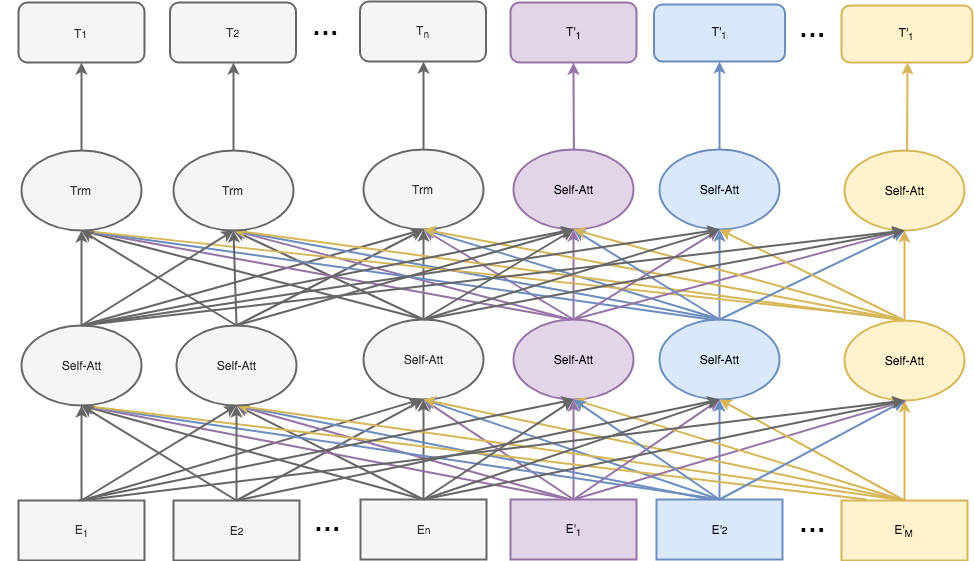
\includegraphics[width=0.95\linewidth]{fig/architecture.png}
    \vspace{20pt}
    \caption{\BertMWE architecture illustration. Grey nodes denotes the original self attention network. Nodes colored in purple, blue and yellow denotes the additional blocks corresponding to specific MWEs.}
    \vspace{10pt}
    \label{fig:variational}
\end{figure}


\subsection{Architecture overview}\label{sec:arch-overview}
In this work we assume that each input text instance are represented as a sequence of tokens $(w_1, ..., w_n)$,
and in addition, there are a set of candidate multi-world expressions $(w'_1, ..., w'_m)$, each corresponds to a span in the original token sequence, with starting index $(st_1, ..., st_m)$, and ending index $(end_1, ..., end_m)$. 

In typical self-attention network such as the original Bert model \cite{devlin2018bert}, the first step is to transform the input sequence into an unordered set, 
and the original position information is captured using the position embedding mechanism \cite{vaswani2017attention}. which on a high level, can be described as representing the input into the form of a permutation invariant set $\{u_1, ..., u_n\}$, where each element $u_i=(w_i, pos_i)$ include both the token $w_i$ and its position $pos_i$, in this case it index in the original sequence $i$.

As illustrated in \autoref{fig:variational}, each element in the input then go through the embedding layer and represented as a set of permutation invariant embeddings vectors $\{E_1, ..., E_n\}$, 
\cite{vaswani2017attention}
and then go through certain numbers of inter-connected self-attention layers, and finally go   to be mapped to the final output layers
$\{T_1, ..., T_n\}$
through some final layers of transformation the's suitable for the specific tasks at hand,  such as sequence labeling and classification \cite{devlin2018bert}.

In \BertMWE, we inject multiword expression into the network in an \textit{homogeneous} fashion: we insert the MWE as additional elements into the input, while the model architecture for processing these input stay the same. 

Specifically, given a set of candidate multi-world expressions $(w'_1, ..., w'_m)$, 
we will similarly transform them into a set of candidate multi-world expressions $(u'_1, ..., u'_m)$, where each element $u_i=(w'_i, pos'_i)$ include the mwe $w'_i$ and its location, which is derived as a function of the span location $f(st_i, end_i)$ in the original sequence $pos'_i$ \footnote{in this work we use the simple average function $f(st_i, end_i) = \lceil \frac{st_i, end_i}{2} \rceil $}.
Then, analagously, we embed the multi-world expressions $(u'_1, ..., u'_m)$ into embeddings vectors $\{E'_1, ..., E'_m\}$.
As shown in \autoref{fig:variational}, the embedding vectors $\{E'_1, ..., E'_m\}$ are concated  with the original vectors, and the newly concatenated set vectors 
$\{E_1, ..., E_n, E'_1, ..., E'_m\}$ are in the exact same form of the original input and fed to the exact same model as before.

The challenge with this approach, however, is that we don't know how many of the candidate MWEs are truly non-compositional and are important for capturing the meaning of the text and best support downstream prediction tasks:
Simply adding all of them into the original tokens' embedding would potentially introduce large amount of noise to the data and obfuscate the original inputs. Blindly ignoring some candidates might miss important non-compositionality information.
we need a way to distinguish good from the bad, and dynamically infer the non-compositionality, along with the set of parameters contained in the deep self-attention networks architecture.


We formualte this using a principled bayesian probabilistic framework. 
Given a dataset $\mathcalD$ containing a set of $N$ observations of tuples $(x,y)$,  $x$ is the input text and $y$ is the target labels of interest ,
if we use  $m_{MWE}$ to denote the model to select from the set of candidate multi-world expressions the true non-composable MWEs to be included in the final model, and 
$m_{Bert}$ to denote the original self attention network that predict the target output from the inputs, the task can then be formally described as a posterior probability inference over the space of all possible models $m_{MWE} \in M_{MWE}, m_{Bert} \in M_{Bert}$, as the following
\begin{align*}
\small
\begin{split}
    P(m_{MWE}, m_{Bert} | \mathcalD) = \frac{  P( \mathcalD | m_{MWE}, m_{Bert} ) P(m_{MWE}, m_{Bert})  }{ \int \int P( \mathcalD | m_{MWE}, m_{Bert} ) P(m_{MWE}, m_{Bert}) }\\
\end{split}
\end{align*}


\subsection{variational parameterization}


\begin{figure}[tb]
    \centering
    \includegraphics[width=\linewidth]{fig/variational_inference.png}
    \vspace{20pt}
    \caption{Graphical model representation for the proposed variational distribution. Plates represent replications over each possible MWEs and each data instances. Empty nodes denotes the latent variables and solid nodes denotes observed data. The latent variables are instantiated and resulted in a neural network, into which the input is passed to and the output is collected. }
    %\vspace{10pt}
    \label{fig:variational}
\end{figure}


The above inference problem is intractable because of the computing the true posterior distribution involves integrals over all possible model spaces which is computationally intractable. 
Instead, we follow  variational inference principle \cite{} to approximate the model posterior with a family of variational distribution $\mathcal{Q}$ over the models, and the goal is to find find a specific distribution $q(m_{MWE}, m_{Bert}) \in \mathcal{Q}$ that are closest to the exact posterior distribution $P(m_{MWE}, m_{Bert} | \mathcalD)$.
We will first describe our choice of the variational family $\mathcal{Q}$, and then continue to specify the variantional inference procedure.


The goal of the \BertMWE is to learn to capture both the individual non-compositionality from the MWEs while fully utilize the modeling power of the deep self-attention network. To that end we propose the a procedure to parameterize our distribution family $\mathcal{Q}$, 
as a probabilistic generative process. 
The basic idea is to view the output target as a mixture of possible models applied to the given input x, 
while including the selection of MWEs as integrated part of the network architecture.
The decision for the inclusion of MwEs is make in a hierarchical manner by a global factor controlling the joint quality of the MWE architecture as well as independent qualities for each MWE.

Specifically, we assuming the network is described by of mean parameter matrixes $W$, and a prior distribution for Bernoulli variables, parameterized by $\Pi$ and $\p_i$ where $i$ range across of the vocabulary of all possible MWEs $v$. The generation process can be described as
\begin{enumerate}
    \item Initialize the network $\Theta$ to skip any MWE in the input by multiplying correspondings parameters in $W$ by zero
    \item Choose global mwe decision variable 
        $b \sim \mbox{Bernoulli}(\Pi)$
    \item{for each MWE in the vocabulary $V$}
    \begin{enumerate}
        \item draw a decision variable $\beta_i \sim \mbox{Bernoulli}(\pi_i)$ for that MWE 
        \item{unmute the MWE parameters in model $\Theta$ only if $s_{j}=1$ and $s_{j}=1$}
    \end{enumerate}
    \item{Choose token $y_{di} \sim \mbox{Mult}(p(x))$}
\end{enumerate}


We can also represent \BertMWE model using the the probabilistic graphical notation, as shown in \autoref{fig:variational}. 
On the top levels are parameters $\Pi$ and $\pi_i, i \in V$, $W$, which are corpus level parameters. Then for each of the $N$ training instance, the set of Bernoulli latent variables
$B$, $\beta_i, i\in v$ are drawn, from which we obtain a specific instantiation of the neural network with parameters $\Theta$. And finally, we pass the input $x$ through the neural network, and outcome of the neural network is generated.


If we denote $\Theta = \{\Theta_{Bert-MWE}, B, \{\beta_i | i \in V\} \vert x,y \in \mathcalD \}$ as the latent variable for the model configurations for each instance in the data, and $Q(\Theta | W, \Pi, \{\pi_i | i \in V\})$ it variational distribution given  
the Bernoulli parameters $\Pi$ and $\pi_i$, and the mean parameter matrices $W$,
The expected log likelihood for the observed data $\mathcalD$ over all the possible configurations can be specified as 
\begin{align}
& \mathbb{E}_{\Theta \sim Q} \log P (\mathcalD | \Theta) \nonumber\\ 
= & \sum_{x, y \in \mathcalD} \int_{\Theta} \log p(y \vert f^{\Theta}(x)) Q(\Theta | W, \Pi, \{\pi_i | i \in V\}) \nonumber\\ 
= & \sum_{x, y \in \mathcalD} \int_B \int_{\beta_i}\int_{\Theta_{Bert-MWE}} \log ( p(B | \Pi) \prod_i^{V} p(\beta_i | \pi_i) \nonumber\\ 
& \quad \quad \quad \quad p(\Theta_{Bert-MWE} \vert W, B, \{\beta_i, i \in V\}) \nonumber\\ 
& \quad \quad \quad \quad p(y \vert f^{\Theta_{Bert-MWE}}(x)) )
\label{eq:exp}
\end{align}

where the conditional distribution 
$p(B | \Pi)$, $p(\beta_i | \oi), i\in v$ are given by the Bernoulli distribution with $\Pi$ and $\pi_i, i\in v$ being the mean parameter, 
$p(\Theta_{Bert-MWE} \vert W, B, \{\beta_i, i \in V\})$ specifies the outcome of zeroing and unzeroing the networks weights $W$ according to the Bernoulli variable $B, \{\beta_i, i \in V\})$ as described by the generative process above,
and finally $p(y \vert f^{\Theta}(x))$ describes the predicted probability of the network as parameterized by $\Theta$ for the target output $y$ given input text $x$. 




Following the variantional inference principle, our goal is then to optimize the parameters for the variational distribution to make it as close to the true model posterior as possible. Specifically, we aim to optimize the the evidence lower bound (ELBO) for the marginal log likelihood of the data $\log P( \mathcalD )$: 
\begin{align}
    &\log P( \mathcalD ) \nonumber\\
    = & \int_{M_{Bert}} \int_{M_{Bert}} \log P( \mathcalD | m_{MWE}, m_{Bert} ) \nonumber\\
    \geq& \mathbb{E}_{\Theta \sim Q} \log P (\mathcalD | \Theta) - D_{KL}(Q( \Theta) ||\mathcal{P}( \Theta)) \nonumber\\
    = & \mathcal{L}_{Bernoulli} (W, B, \{\beta_i, i \in V\}) \label{eq:elbo0}
\end{align}

where $\mathbb{E}_{\Theta \sim Q} (P (\mathcalD | \Theta) )$ is the expectation of the conditional likelihood under the variational distribution as described in \autoref{eq:exp}, and the KL divergence between the variational distribution and the prior distribution of the model parameters $\mathcal{P}(\Theta)$, $D_{KL}(Q( \Theta) ||\mathcal{P}( \Theta))$ can be approximated  as in \cite{gal2016uncertainty}.
%
%, we omit this term in practise and focus on optimizing the likelihood term  $\mathbb{E}_{\Theta \sim Q} (P (\mathcalD | \Theta) )$.


%Following the variational interpretation, dropout is seen as an approximating distribution $q_\theta(\bo)$ to the posterior in a Bayesian neural network with a set of random weight matrices $\bo = \{\W_l\}_{l=1}^L$ with $L$ layers and $\theta$ the set of variational parameters. 
% Assume that the weight matrices can be written as $\bo = g(\theta, \bepsilon)$ with $\epsilon$ a random variable that does not depend on $\theta$.
%The optimisation objective that follows from the variational interpretation can be written as:

\subsection{efficient approximate inference}\label{sec:approximate-inference}


In order to evaluate the derivative and optimize the ELBO (see \autoref{eq:elbo0}) without exact integration over the latent variables, 
we resort to sampling based methods 
that approximate the derivative value by drawing samples from the variational distribution \cite{ranganath2014black}. 
However, directly sampling from the distribution, e.g. through stochastic gradient variational bayes  \cite{rezende2014stochastic} might be hard due to high variance in the estimated gradients and the sheer amount of latent variables \cite{kingma2015variational}.
We instead leverage the local re-parameterization trick \citep{Kingma2015} to  
decompose the global sample uncertainty in the model weights into local noise, and remove the correlation between samples in the mini-batch.

Another challenge is that, because the generation process follows a Bernouli distributions, 
which is discrete and thus block the back-propagation from the estimated likelihood, 
it is very hard for us to obtain gradients about the variational parameters and re-adjust the distribution. 
One possible approach is to relax the discrete distribution into a continuous, Gaussian distribution \cite{wang2013fast, chen2019large}. However, these two families of distributions are of very different nature and 
requires significant hand tuning such as truncating in order  to prevent the computation from diverging, and in practice cause the model to underperform \cite{molchanov2016dropout}, not to mention that fact the computation error could accumulate as the number of layers increases, and more  approximation is applied for each layer. 

To remedy this, we adopt the Gumbel-Max trick \cite{gumbel1954statistical, gummaddison2014sampling} as the continuous relaxation of the bernoulli distribution
and %follow Jang. et.al. \cite{jang2016categorical} to use the softmax function as a continuous relaxation to 
make the sample differentiable with respect to the variational parameter. 
Specifically, the continuous relaxation to Bernoulli distribution with mean parameters $p$ can be parameterized as
\begin{equation}
Gumble_{t}( \tilde{\beta} | p) = t \left( \frac{p}{\tilde{\beta}^t} + \frac{1 - p}{(1- \tilde{\beta})^t} \right)^{-2} 
\frac{p}{\tilde{\beta}^{(t + 1)}} \frac{1 - p}{(1 - \tilde{\beta})^{(t + 1)}}  
\\
\end{equation}
where $t$ is the "temperature" parameter that controls how close the continuous relaxation is to the Bernoulli distribution, when it approach 0, the resulted $y$ recovers the original Bernoulli distribution.

For Bernoulli random variable with mean parameter $\pi$, this amounts to drawing a uniform random variable  $u \sim \Unif (0, 1)$ and compute the sampled value $z$
 through a sigmoid function \cite{gal2017concrete}
\begin{align}
\tilde{\beta} &= \text{sigmoid} \bigg(
\frac{1}{t} \cdot \big(
\log \pi
- \log (1 - \pi)
+ \log u
- \log (1 - u)
\big)
\bigg) \label{eq:gumbel-sample}
\end{align}


%For distributions that are reparameterizable, we can compute the sample $z$ as a deterministic function $g$ of the parameters $\theta$ and an independent random variable $\epsilon$, so that $z = g(\theta, \epsilon)$. The path-wise gradients from $f$ to $\theta$ can then be computed without encountering any stochastic nodes:
%\begin{equation}
%\frac{\partial}{\partial \theta} \mathbb{E}_{z\sim p_\theta}\left[f(z))\right] = \frac{\partial}{\partial \theta} \mathbb{E}_{\epsilon}\left[f(g(\theta,\epsilon))\right] = \mathbb{E}_{\epsilon\sim p_\epsilon}\left[\frac{\partial f}{\partial g} \frac{\partial g}{\partial \theta}\right]
%\end{equation}




Without loss of generality, we consider the case where the discrete variables $B$ and $\{
\beta_i | i \in V\}$ are directly replaced with Gumbel-softmax distributed continuous relaxation counterpart, denoted $\tilde{B}$ and $ \{ \tilde{\beta}_i  | i \in V\}$, and 
we apply these quantities multiplicatively into the model weights for the corredponding MWEs to obtain the resulted model parameters, 
instead of completing zeroing them out, or keeping them at 100\%.
Denoting $\tilde{\Theta} = \{\Theta_{Bert-MWE}, \tilde{B}, \{\tilde{\beta}_i | i \in V\} \vert x,y \in \mathcalD \}$, and $ \tilde{Q} (\Theta | W, \Pi, \{\pi_i | i \in V\})$ as its variational distribution, the expected conditional log likelihood for the observed data $\mathcalD$ can then be re-written as
\begin{align}
& \mathbb{E}_{\tilde{\Theta} \sim \tilde{Q}} \log P (\mathcalD | \tilde{\Theta}) \nonumber\\ 
= & \sum_{x, y \in \mathcalD} \int_{\tilde{B}} \int_{\tilde{\beta}_i}\int_{\Theta_{Bert-MWE}} Gumble(\tilde{B} | \Pi) \prod_i^{V} \log ( Gumble(\tilde{\beta}_i | \pi_i) \nonumber\\ 
& \quad \quad \quad \quad p(\Theta_{Bert-MWE} \vert W, B, \{\beta_i, i \in V\}) \nonumber\\ 
& \quad \quad \quad \quad p(y \vert f^{\Theta_{Bert-MWE}}(x)) )
\label{eq:exp-gumble}
\end{align}

Our goal then becomes to optimize the evidence lower bound indicated by the above expected conditional log likelihood 

\begin{align}
    &\log P( \mathcalD ) \nonumber\\
    \geq& \mathbb{E}_{\tilde{\Theta} \sim \tilde{Q} } \log P (\mathcalD | \tilde{B}, \tilde{\Theta})  - D_{KL} ( \tilde{Q} ( \tilde{\Theta}) ||\mathcal{P}( \tilde{\Theta} )) \nonumber\\
    = & \mathcal{L}_{Gumble} (W, B, \{\beta_i, i \in V\}) \label{eq:elbo0}
\end{align}

The first term in the ELBO refers to the expected conditional log likelihood of the data, as defined in \autoref{eq:exp-gumble}, and the second term is the KL divergence between the new variational distribution $\tilde{Q} ( \tilde{\Theta})$ 
and a predefined prior distribution  $\mathcal{P}( \tilde{\Theta})$.
Although we can analytically approximate it by again following \cite{gal2016uncertainty}, 
in practise we ignore this term because it is $O(N)$ orders of magnitude smaller than the expected conditional likelihood, where $N$ the amount of data to train the model. This is especially true when we can train the models weights using very large amount of training instances, for example from the unsupervised text data under the language modeling objective \cite{devlin2018bert}.





\begin{figure}[htb]
    \centering
    \includegraphics[width=0.95\linewidth]{fig/model_architecture.png}
    \vspace{20pt}
    \caption{mwe dropout is applied at each level of architecture, as a result,
    if dropout is zero, will completelty dropout the entire ff need, not just one single layer
    . reduce back to original structure.  If kept will be treated the same.
    interference can be limited to only low level embedding layers, }
    \vspace{10pt}
    \label{fig:architecture-mwe-dropout}
\end{figure}


%ied the dropout for each multi-word together
%will drop out the entire 


% Here we follow a similar approach to \citep{Kingma2015}, and rely on the variational interpretation of discrete dropout in order to obtain a principled optimisation objective \citep{Gal2016Uncertainty}.


\subsection{Network architecture}
Finally, we describe the architecture design to fully specify the  variational distribution of model parameters $p(\Theta_{Bert-MWE} \vert W, B, \{\beta_i, i \in V\})$. 
The challenge is that approximate inference scheme no longer treats the selection of MWEs as black or white decisions and the non-compositionality inference needs to be dynamically integrated into the model architecture. 
% To that end, we propose the following neural network design that inject the approximate inference over the selection of MWEs, as controlled by $B, \{ \beta_i | i \in V \}$, and the self-attention network parameters, $W$ into one single architecture.


%because we're trying to estimate the "dropout" probability $\Pi$ and $\{\pi | i \in V\}$ associated with each MWEs, we need to estimate its gradient and therefore can no longer considering the MWEs as black and white and instead resort to the 


Our proposed architecture is shown in \autoref{fig:architecture-mwe-dropout}. 
Given one instance of input text, the first step is to embed the discretized tokens into vector representations to feed into downstream neural networks.
For single word embedding, this amounts of combining the token embedding, position embedding and sentence level information into 
a set of word embedding vectors $\{E'_1, ..., E'_m\}$ corresponding to each token, for which we follow the exact same implementation as in \cite{devlin2018bert}.

In addition to embedding the single words, 
we perform MWE embedding, which yields two outcomes.
The first is a set of vectors $\{E'_1, ..., E'_m\}$, analogous to the single word embedding, 
by following the procedure described in section \autoref{sec:arch-overview}. 
Secondly, we obtain the "dropout" rate $\bm{\beta} \triangleq [\beta_1, ..., \beta_m]^T$ for each corresponding MWE 
by sampling from the Gumbel-softmax distribution (See \autoref{eq:gumbel-sample}), which is specified by the corresponding variational parameters $\{\pi_i \vert i \in V\}$.

% Assume that the set of variational parameters for the dropout distribution satisfies $\theta=\{\M_l, p_l\}_{l=1}^L$, a set of mean weight matrices and dropout probabilities such that $q_\theta(\bo) = \prod_l q_{\M_l}(\W_l)$ and $q_{\M_l}(\W_l)=\M_l \cdot \diag[\text{Bernoulli}(1-p_l)^{K_l}]$ for a single random weight matrix $\W_l$ of dimensions $K_{l+1}$ by $K_l$.


Next, we concatenate the single word embeddings and MWE embeddings together, as
a matrix $\mathbf{E} \triangleq [E_1; ...; E_n| E'_1; ...; E'_m]$ to be used as the input to the downstream self-attention network layers, 
in the exact same form as the resulted embedding in the original architectures
\cite{vaswani2017attention}.




%Along with the embedding, we perform a stochastic lookup, to sample the characteristic MWE "dropout" ratio $\beta = [\beta_1, ..., \beta_m]^T$ associated with each of the MWE, To match the shape of the embedding, we extend the dropout ratio to single tokens, by prepending $1$s to the ratio, as $\bar{beta} \triangleq x [\mathbbm{1}_n^T | \beta]$, where $\mathbbm{1}_n$ denotes a length $n$ vector containing all 1s.

In order to apply the MWE selection from sampled MWE "dropout" rate $\bm{\beta}$, a simple dropout over the the embedding matrix is not sufficient, because the network architecture has changed according to the input embedding dimension, 
and may eventually diverge further and further as the input is passed through the whole network.

To remedy this we propose a novel dropout scheme called "tied architectural dropout", that dropout the a set of related weights across the entire neural networks, simultaneously controlled by the same sampled dropout ratio.
Specifically, we apply an MWEDropout layer 
before each of the repeated transformer blocks\cite{devlin2018bert}
to implement the selection of MWEs, where the characteristic "dropout" ratio are used to scale down the hidden states for the corresponding MWEs, and the hidden states for single words are left intact.  
Specifically, we compute MWEDropout from the input hidden states $\mathbf{H}$ and the MWE dropout ratio $\bm{\beta}$. 
The output can be specified as 
\begin{equation}
   \mathrm{MWEDropout}(\mathbf{H}, \mathbf{\beta}) =  diag([\bm{{\mathbbm{1}}}_n \vert \bm{\beta}]) \cdot \mathbf{H}
\end{equation}
where $\bm{{\mathbbm{1}}}_n$ denotes an $n$ dimensional vector filled with 1s.

The MWE-Dropout layer is then followed by the Multi-Head Attention, LayerNorm, FeedForward and another LayerNorm layer, for each transformation block, exactly as in the original architecture \cite{vaswani2017attention}. This newly grouped Bert-MWE transformer block, is then stacked repeatedly for $N$ times and finally fed into donwstream prediction heads, in the exact same way as \cite{devlin2018bert}.




\subsection{Prediction} \label{sec:prediction}
The goal of variational inference is to obtain the hyper-paramters governing $\Pi, \{\pi_i \vert i \in V\}$ the as well as the mean-weights $W$ that jointly controls the probability distribution of model parameters $B, \{b_i \vert i \in V\}, \Theta_{Bert-MWE}$, the task now is to predict the target output given a new incoming input text $x$.
Instead of performing  from a static point estimate of the model, we perform prediction by directly drawing samples from posterior predictive distribution.

Specifically, the posterior predictive distribution of $y$ under the variational distribution $\tilde{Q}$ can be obtained by computing the expectation of the model parameters $\tilde{\Theta}$ under all possible model settings
\begin{align}
& \mathbb{E}_{\tilde{\Theta} \sim \tilde{Q}} P (y | x, \tilde{\Theta}) \nonumber\\ 
= & \int_{\tilde{B}} \int_{\tilde{\beta}_i}\int_{\Theta_{Bert-MWE}} Gumble(\tilde{B} | \Pi) \prod_i^{V} Gumble(\tilde{\beta}_i | \pi_i) \nonumber\\ 
& \quad \quad \quad \quad \quad \quad \quad \quad p(\Theta_{Bert-MWE} \vert W, B, \{\beta_i, i \in V\}) \nonumber\\ 
& \quad \quad \quad \quad \quad \quad \quad \quad p(y \vert f^{\Theta_{Bert-MWE}}(x)) 
\label{eq:exp-gumble}
\end{align}

In terms of neural network architecture, this amounts to keeping the exact same Gumble-softmax sampling operation (\autoref{eq:gumbel-sample}) and the same behavior of the MWE dropout layer during both training and inference stage. Intuitively, this is because the learned model distribution are shared across the training and inference.
%!TEX root =  concept_mining.tex


\begin{table*}
\small
\centering
\begin{tabular}{llllll} 
\toprule
Datasets & Task & Domain & Metric & $\vert$ Train$\vert$ & $\vert$Test$\vert$  \\
\midrule

Sample Text & \multirow{5}{*}{\begin{tabular}[c]{@{}l@{}}Text Modeling\end{tabular}}  & General text           & \multirow{5}{*}{\begin{tabular}[c]{@{}l@{}}Word prediction + \\ Next sentence prediction\end{tabular}} & 16   & 480     \\
Sample Large &                         & General text &       & 280K  & 8.4M     \\
Wikitext-2 converted       &                         & Articles from Wikipedia &   & 60K  & 1800K     \\
Arxiv Computer Science      &                         & Technical papers from \url{arxiv.org}  &       & 362K  & 1.1M     \\
Arxiv Math       &                         & Technical papers from \url{arxiv.org} &      & 175K  & 525K     \\
\midrule
CoLA & classification  & Books and journal articles  & Matthews coefficient      & 8.5k & 1k    \\
\midrule
MRPC &  \multirow{2}{*}{\begin{tabular}[c]{@{}l@{}}paraphrase\end{tabular}}  & News &  \multirow{2}{*}{\begin{tabular}[c]{@{}l@{}}Accuracy / F1\end{tabular}} 
& 3.7k & 1.7k   \\
QQP &                         & Questions from Quora &      & 364k & 391k  \\ 
\midrule
STS-B & Sentence Similarity                    & Misc.    & Pearson/Spearman       & 7k & 1.4k  \\
\midrule
MNLI        &  \multirow{2}{*}{\begin{tabular}[c]{@{}l@{}}NLI\end{tabular}}                   & Internet Crawl  & \multirow{2}{*}{\begin{tabular}[c]{@{}l@{}}Accuracy\end{tabular}}      &393k & 20k   \\
RTE      &          & Wikipedia             &      &  2.5k & 3k  \\
\midrule
QNLI     & QA + NLI & News and Wikipedia   & \multirow{2}{*}{\begin{tabular}[c]{@{}l@{}}Accuracy\end{tabular}}      & 105k & 5.4k  \\
WNLI        & coreference + NLI & Fiction books   &        & 634 & 146  \\
\bottomrule
\end{tabular}
\caption{An overview of the benchmark datasets used for different tasks along with their description and statistics}
\label{tab:dataset}
\end{table*}





\begin{figure*}
\begin{minipage}[b]{.5\linewidth}
 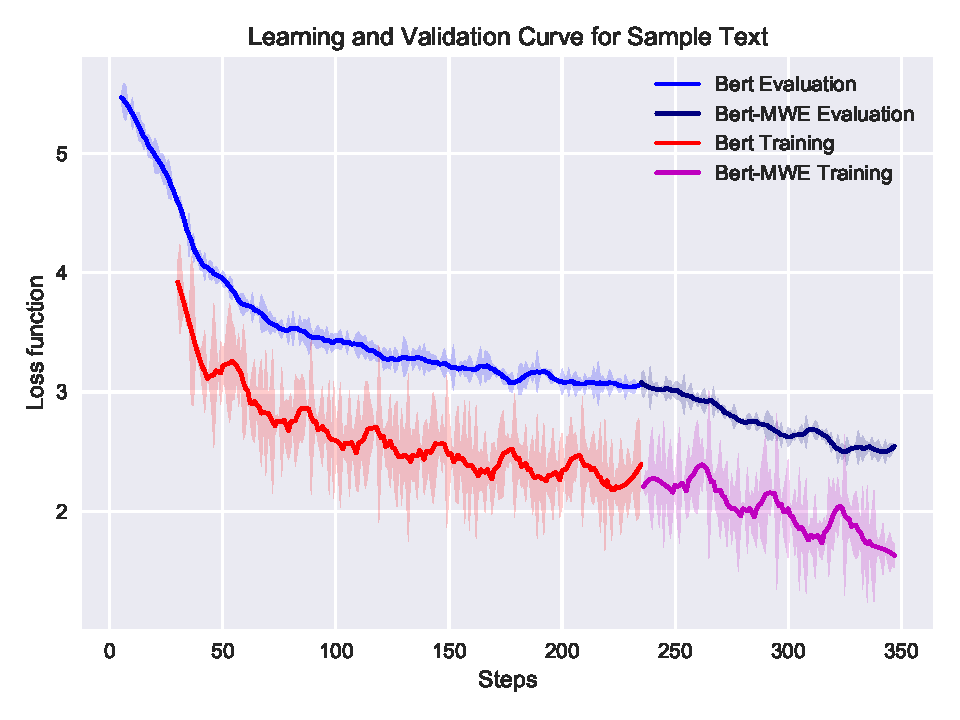
\includegraphics[width=\linewidth]{fig/st.pdf}
\label{fig:manual-eval1}
\end{minipage}
\begin{minipage}[b]{.5\linewidth}
 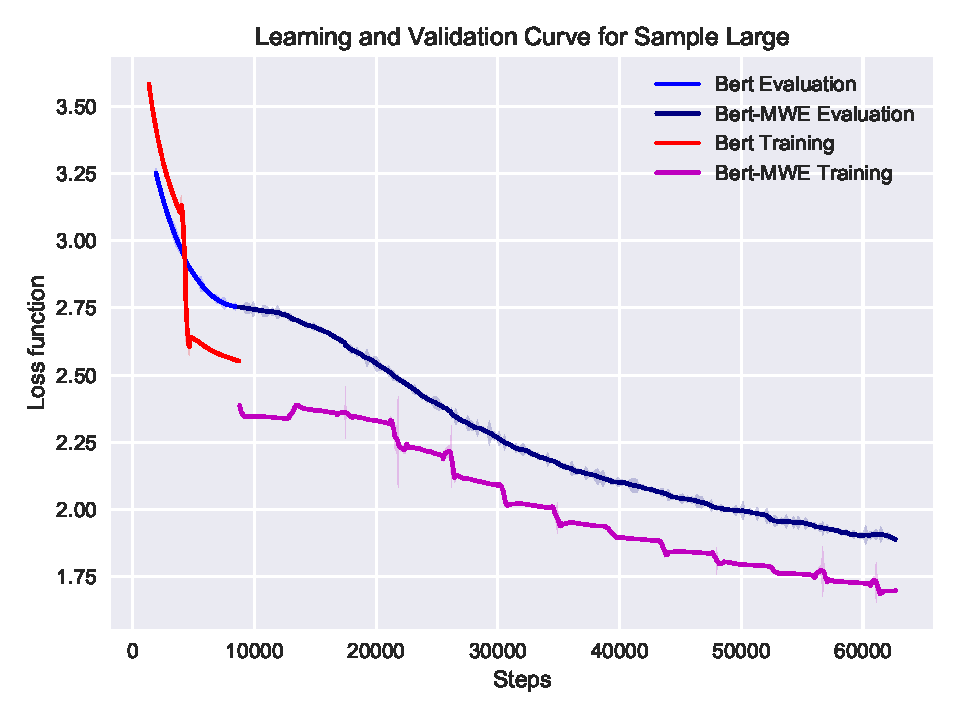
\includegraphics[width=\linewidth]{fig/sl.pdf}
\label{fig:manual-eval2}
\end{minipage}
\vspace{-15pt}
\caption{Learning and validation curve for the text modeling task}
\label{fig:learning-curve}
%\vspace{3pt}
\end{figure*}





\begin{table*}
\begin{center}
\begin{tabular}{lllclcllc} 
\toprule
System      & CoLA                                                                         & MRPC                                                                              & QQP                           & STS-B              & QNLI                     & MNLI          & RTE           & WNLI                      \\ 
\hline
BiLSTM      & 11.6                                                                         & 81.8/74.3                                                                         & \multicolumn{1}{l}{62.5/84.2} & 70.3/67.8          & \multicolumn{1}{l}{74.6} & 65.6          & 57.4          & \multicolumn{1}{l}{65.1}  \\
BiLSTM+Attn & \textcolor[rgb]{0.133,0.133,0.133}{\textcolor[rgb]{0.133,0.133,0.133}{18.6}} & \textcolor[rgb]{0.133,0.133,0.133}{\textcolor[rgb]{0.133,0.133,0.133}{83.9/76.2}} & 72.8/70.5                     & 72.8/709           & 74.3                     & 67.6          & 58.4~ ~~      & 65.1                      \\
OpenAI GPT  & 45.4                                                                         & 82.3/-                                                                            & 70.3/-                        & 80.0/-             & 87.4                     & 82.1          & 56.0          & 65.1                      \\
Bert        & 57.9                                                                         & 86.0/89.9                                                                         & 89.9/86.7                     & 89.6/89.2          & 90.8                     & 83.4          & 67.1          & 57.7                      \\
\BertMWE (Simplified)     & 58.1                                                                         & 86.0/89.9                                                                         & 90.7/87.5                     & \textbf{90.0}/89.5 & 91.3                     & \textbf{84.0} & \textbf{72.2} & 56.3                      \\
    \BertMWE        & \textbf{59.7}                                                                & \textbf{86.5/90.4~}                                                               & \textbf{90.9/87.7}            & \textbf{90.0/89.6} & \textbf{91.5}            & \textbf{84.0} & \textbf{72.2} & \textbf{63.4}             \\
\bottomrule
\end{tabular}

   \caption{Performance on supervised label prediction}
   \label{tab:glue_results}
\end{center}
\end{table*}



\section{Experiments}\label{sec:bert_mwe_experiments}

In this section we experimentally evaluate the proposed approach over an wide range of tasks across different domains and demonstrate its effectiveness over the state of the art baseline approaches.




\subsection{Setup}

\noindent \textbf{Hardware Environment}
The model training and prepossessing is conducted on a lab server with 3 
GeForce RTX 2080 GPU card, 2 6-core Intel(R) Core(TM) i7-6800K CPU @ 3.40GHz CPU with 12GB memory. The longest experiments took no more than 3 days.


\noindent \textbf{Model architecture and hyper-parameter settings}
Since the proposed \BertMWE approach is built upon the Bert self-attention network architecture \cite{devlin2018bert},
and 
we're mainly interested in how much it can \textit{improve} upon the basic Bert model, 
we follow the exact same architecture, hyper-parameter and optimizer settings as suggested by 
\cite{devlin2018bert} for each specific tasks 
and refer the reader to the original paper for details about the architecture and parameter.

\noindent \textbf{Model training and weight initialization}
In order to more directly see the difference between the \BertMWE and the original Bert model, we conduct the model training of \BertMWE in an \textit{incremental} fashion:
we first follow the best training settings for each different variant of the Bert model  to train the basic model for a specific downstream task; after that, we start to train the corresponding \BertMWE 
for the Bert variant, and use the trained Bert model to initialize the \BertMWE. In other words, \BertMWE only changes the original Bert model with addition MWE structure, but retains all the trained weights.

\noindent \textbf{Model variants}
We apply the \BertMWE approach over the two different variants of Bert model as proposed in \cite{devlin2018bert}: the Bert-Finetune model where we use the pretrained weights as initialization, and fine-tune all layers of the model end to end; and the Bert-Feature model, where we freeze the pretrained  model weights and use the outputted hidden states as feature to train a task specific prediction head. 

We also 
explore two different variants of applying the non-compositionality.
The first is the theoretically sounded \BertMWE, which fully follows the variational inference procedure and learns a distribution over all possible models for prediction, as shown in \autoref{sec:var-param}; The second is a simplified version, 
 \BertMWE (Simplified), 
which do not add the \textit{MWE Dropout} layer to the network to explicitly utilize variational inference. 
However, it may still conduct inference over the importance of multi-word expressions to some extent by dynamically scale their inputted embedding to the downstream network.

\subsection{Text modeling} \label{sec:dataset}
We first evaluate the proposed approaches on on the task of modeling text data.
Specifically, we follow the construction of masked language model and next sentence prediction task \cite{devlin2018bert} to create our training and additionally a separate evaluation set, 
which shares no overlap with the training set. 
To make the competition fair with original Bert models, 
we will discard from the input text any MWEs that has overlaps with the masked position. 


We evaluate our approach over the following corpus. The dataset statistics are shown in \autoref{tab:dataset}. 


\begin{table*}[thbH]
\centering
\small
\begin{tabular}{lcccccc} 
\toprule
Datasets                                  & Training strategy                & Methods   & Evaluation~Loss ~ & Improvement            & ~Training Loss~        & Improvement              \\ 
\midrule
\multirow{6}{*}{Sample Text} & \multirow{2}{*}{Bert Finetune} & Base   & 0.39                & -                      & 0.001                     & -                        \\
                                               &                                & \BertMWE         & 0.290                & -25.7\%           & 0.000            & -66.7\%              \\
\cline{2-7}
                                               & \multirow{2}{*}{Bert Feature}  & Base  & 3.272                & -                      & 2.074                     & -                        \\
&                                & \BertMWE      & 2.35                & -28.2\%                      & 1.139                     & -45.1\%                       \\ 
\midrule
\midrule
\multirow{6}{*}{Sample Large} & \multirow{2}{*}{Bert Finetune} & Base   & 2.768                & -                      & 2.552                     & -                        \\
                                               &                                & \BertMWE      & 1.866                & -32.1\%                      & 1.670                     & - 34.56\%                       \\ 
\cline{2-7}
                                               & \multirow{1}{*}{Bert Feature}  & Base & 3.991                & -                      &         3.712            & -                        \\
                                               &                                & \BertMWE         & 3.918                 & -1.8\%           & 3.654            & -1.6\%              \\
\midrule
\midrule
\multirow{6}{*}{WikiText-2} & \multirow{2}{*}{Bert Finetune} & Base   & 1.851                & -                      & 0.588                                & -                        \\
&                                & \BertMWE      & 1.390                & -24.9\%                      & 0.489          & -16.8\%                       \\ 
\cline{2-7}
                                               & \multirow{2}{*}{Bert Feature}  & Base & 2.700                & -                      & 2.511                     & -                        \\
                                               &                                & \BertMWE         & 2.669                & -1.1\%           & 2.491            & -0.8\%              \\
\midrule
\midrule
\multirow{6}{*}{Arxiv CS} & \multirow{2}{*}{Bert Finetune} & Base   & 2.560                & -                      & 2.336                     & -                        \\
                                               &                                & \BertMWE      & 2.137                & -16.5\%                      & 1.859                     & -20.4\%                       \\ 
\cline{2-7}
                                               & \multirow{2}{*}{Bert Feature}  & Base & 3.306                & -                      & 3.072                     & -                        \\
                                               &                                & \BertMWE         & 3.277                & -0.9\%           &  3.049            & -0.7\%              \\
\midrule
\midrule
\multirow{6}{*}{Arxiv Math} & \multirow{2}{*}{Bert Finetune} & Base   & 1.658                & -                      & 1.399                     & -                        \\
                                               &                                & \BertMWE      & 1.649                & -0.5\%                      & 1.399                     & -0\%                       \\ 
\cline{2-7}
                                               & \multirow{2}{*}{Bert Feature}  & Base & 3.131                & -                      & 2.928                     & -                        \\
                                               &                                & \BertMWE         & 3.024                & -3.4\%           & 2.813            & -3.9\%              \\
\midrule
\bottomrule
\end{tabular}
\caption{Experiment results on text modeling}
\label{tab:text_modeling}
\end{table*}





%We follow the original pre-training procedure for finetuning and evaluating different approaches, by first pre-processing the input corpus following the mask-sample-replace procedure for training the masked language model, and using the the sum of the mean masked LM likelihood and mean next sentence prediction likelihood as the objective function. 
%In order to have a fair comparison for the MWE based approaches, we prevent the information "leakage" from the MWE in the sentence that may contain the masked tokens, by discarding in the masking stage any MWE in the input if there is any overlap between the MWE and the masked tokens. The evaluation metric is then obtained by measuring the same objective function as in the training set as in a separate evaluation set.
%We carry out the text modeling task capability over several representative dataset across various domains, as described by the datasets listed below. 


%We have collected the following corpus, covering the domain of computer science, physics \& mathematics and medicine.
% The statistics of these datasets are summarized in Table S1, and the details are described below.

\noindent \textbf{Sample Text} 
We first verify our approaches over a simple 30-sentence corpus
obtained from the widely adopted Pytorch implementation of Bert repository \footnote{\url{https://github.com/huggingface/pytorch-pretrained-BERT/blob/master/samples/sample_text.txt}}.


\noindent \textbf{Sample Large}
The Sample Large corpus is also provided by Pytorch Bert repository  \footnote{\url{https://github.com/huggingface/pytorch-pretrained-BERT/blob/master/samples/sample_text.txt}}
which consists of about 500K natural language text to evaluate of our approaches in a large scale setting.
\footnote{\url{https://ext-bert-sample.obs.eu-de.otc.t-systems.com/small_wiki_sentence_corpus.txt}}

\noindent \textbf{WikiText-2} 
The WikiText-2 corpus is a cleaned Wikipedia corpus proposed by Merity et.al \cite{merity2016pointer} as a standard benchmark for language modeling in the general domain. 

\noindent \textbf{Arxiv Computer Science} We evaluate our approaches for modeling text from technical domains, 
which is obtained by collecting the titles and abstracts of 70K papers from the open access repository \url{arxiv.org} under the top level category of computer science from the year of 2008 to 2018. 


\noindent \textbf{Arxiv Maths} 
We evaluate our approach over another 
technical domain, by collecting the titles and abstracts of 65K papers  from \url{arXiv.org}, under the top level category "mathematics". 

\subsection{Supervised label prediction}
we then evaluate the proposed approaches over an array of tasks that will take the text as input and learn to predict additional supervision labels to solve downstream analytical tasks. 
For this we follow the standard setting from 
General Language Understanding Evaluation (GLUE) \cite{wang2018glue}, which is a collection of many supervised label prediction tasks for natural language text.
Since GLUE does not distribute labels for the Test set and original evaluation was measured on the dev set \cite{devlin2018bert}, we use the dev set' evaluation results as the performance metric.
Specifically, we choose to evaluate our methods over the following dataset.

\noindent \textbf{CoLA} The Corpus of Linguistic Acceptability is a binary classification task where given a single sentence, the goal is to predict whether it is grammatically acceptable. We follow the author \cite{wang2018glue} and use Mathews correlation coefficient as the evaluation metric.

\noindent \textbf{MRPC} The Microsoft Research Paraphrase Corpus is a collection of sentence pairs from online news sources for paraphrase detection. Given a pair of sentence, the goal is to predict whether they are semantically equivalent. 
Because the classes are imbalanced, we use both accuracy and F1 score as the performance metric.


\noindent \textbf{QQP} The Quora Question Pairs dataset is another text similarity dataset consisting of pairs of questions from Quora, which follows the same format as \textbf{MPRC}. It also has imbalanced classes and therefore both accuracy and F1 score are reported.


\noindent \textbf{STS-B} 
The Semantic Textual Similarity Benchmark is yet another paraphrase detection dataset from news headlines,  video and image captions for natural language inference. Specifically, given a pair of sentence, the goal is to predict a score from 1 to 5 measuring the strength of their semantic similarity. We use Pearson and Spearman correlation coefficients as the performance metric.


\noindent \textbf{MNLI} The Multi-Genre Natural Language Inference dataset is a crowdsourced collection of entailment classification data collected by William et.al. \cite{williams2017broad}. 
Given a pair of sentences, the goal is to predict whether the 
second sentence (hypothesis) is an entailment or contradiction of the first one (premise), or it is neither of the above.

\noindent \textbf{QNLI} The Question Natural Language Inference dataset is a converted version of the Stanford Question Answering Dataset where given a pair of question and sentence, the goal is to predict whether the sentence contains the answer to the question.

\noindent \textbf{RTE} The Recognizing Textual Entailment dataset is a collection of text entailment dataset constructed from on news and Wikipedia and is formatted the same way as \textbf{MNLI} .

\noindent \textbf{WNLI} The Winograd Natural Language Inference dataset is converted from Winograd Schema Challenge where the goal is to determine the referent of the pronouns in the given sentence. Given an input pair of sentence, the goal is to predict whether the second sentence is equivalent to the first one, i.e. by replacing the pronoun with the correct referent.




\subsection{Performance evaluation}
\noindent \textbf{Text modeling}
We first evaluate our approach over the task of modeling the text, under the Bert-pretraining objective \cite{devlin2018bert}, the results are shown in \autoref{tab:text_modeling}. We omit the \BertMWE (Simplified) model for clearity because it generate similar performance with the \BertMWE, possibly because it can scale its embedding parameters to simulate the dropout behavior.
We can see from the results that \BertMWE model is able to efficiently utilize the training set, (by reducing the training error), while at the same time significantly reduce the loss on evaluation set on most of the benchmarks. 
The reduction in training and evaluation loss is always in sync with the \BertMWE model, which further confirms that the additional  complexity in \BertMWE compared to Bert model does lead to over-fitting, and in many cases, lets the model learn better structure of the data.

\noindent \textbf{Supervised label prediction}
We evaluate our approaches over the task of predicting the external supervised labels, as shown in table \autoref{tab:glue_results},
where we list the performance for the Bert based models along with several additional baseline methods whose results are obtained from the Glue online leaderboard \footnote{\url{https://gluebenchmark.com/leaderboard/}}.
We can see that \BertMWE is able to build upon the already very strong Bert base model, and achieve statistically significant improvement over a wide range of tasks, and outperform other strong baseline methods.





\subsection{Case study}
To provide further insights about the learning process, we visualize the learning and validation curve for the text modeling datasets used in the performance evaluation, as shown in \autoref{fig:learning-curve}. We can see from the results that, incorporating the additional structure of \BertMWE gives significant impact over the base Bert model, by better exploiting of the training data to greatly reduce the training error, while at the same time generalizing well to the unseen data and keeping the performance in evaluation dataset in sync.



\section{Conclusion}
In this work, 
we propose a principled probablistic framework \BertMWE that builds upon the state of the art 
model for processing text, 
deep self attention network architecture, 
to incorporate the modeling power of the deep self attention network architecture as well as the rich information contained in natural language non-compositionality, 
through a mechanism of 
dynamically adjusting the deep self attention network architecture to inject the non-compositionality information, 
under the variantional inference framework. We performed extensive experiments over a large range of tasks and demonstrated that our approach build up upon the state of the art Bert model and can bring additional significant improvement.
Many future work exists. For example, how can we effectively mine concepts that are best for improve the network performance, in a end-to-end manner? Moreover, how can incorporte further linguistic structure into the network, to make the architecture richer and more meaningful, while keep pushing the boundary in terms of performance? These are all very interesting directions to explore in the future.




\balance

\bibliographystyle{IEEEtran}
\bibliography{conceptBib}
\end{document}
